\section*{Концептуальный дизайн}
Концептуальный дизайн позволяет рассмотреть создаваемую систему с точки зрения пользователей. На рисунке \ref{fig:idef0-1} отображена контекстная диаграмма верхнего уровня, которая обеспечивает наиболее общее или абстрактное описание работы системы. Данный вид диаграммы позволяет формализовать описание запросов пользователя и ответов системы на них, отобразив её в виде <<чёрного ящика>>.

Для уточнения деталей по операции бронирования, отображённой на диаграмме верхнего уровня, используется дочерняя диаграмма, которая изображена на рисунке \ref{fig:idef0-2}. Она определяет последовательность выполнения операций в системе при обработке запроса клиента. 

\begin{figure}[h!]
	\begin{center}
		{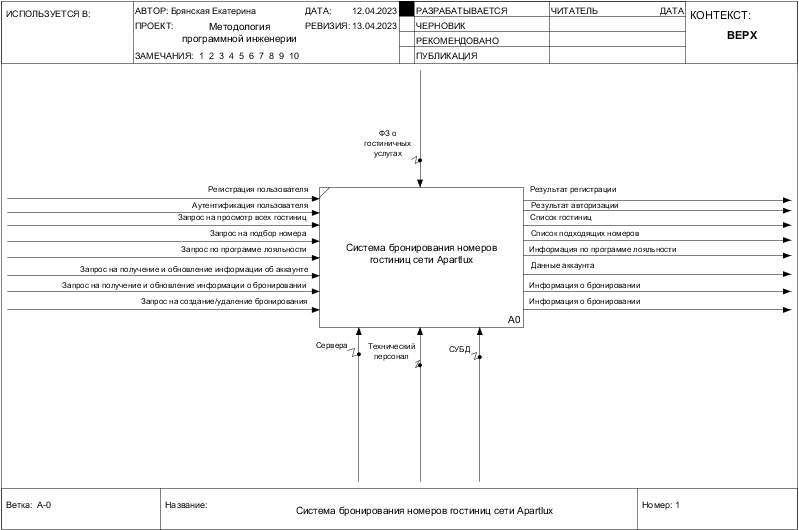
\includegraphics[scale = 0.82, angle=90]{img/idef0/01_A-0.png}}
		\caption{Концептуальная модуль системы в нотации IDEF0.}
		\label{fig:idef0-1}
	\end{center}
\end{figure}

\begin{figure}[h!]
	\begin{center}
		{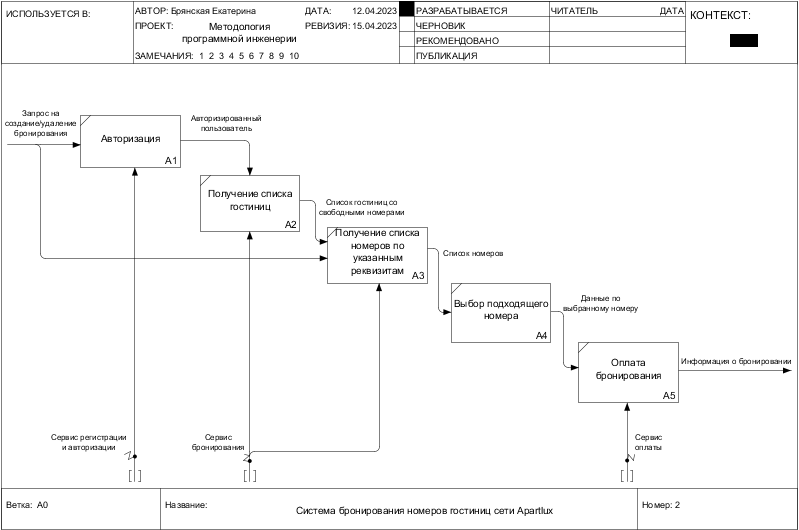
\includegraphics[scale = 0.79, angle=90]{img/idef0/02_A0.png}}
		\caption{Детализированная концептуальная модель системы в нотации IDEF0.}
		\label{fig:idef0-2}
	\end{center}
\end{figure}

\pagebreak

\section*{Сценарии функционирования системы}
\textbf{Регистрация клиента}
\begin{enumerate}
	\item Пользователь нажимает на кнопку <<Зарегистрироваться>> в интерфейсе.
	
	\item Пользователь перенаправляется на страницу, которая содержит поля для заполнения его данных.
	
	\item Пользователь вводит данные в форму и для завершения регистрации нажимает на кнопку <<Готово>>, тем самым подтверждая верность своих данных, а также согласие на их обработку и хранение.
	
	\item Если пользователь с введенным для регистрации логином уже существует, то клиент перенаправляется на страницу ошибки. При успешной регистрации клиент попадает на страницу своего профиля в системе. \\
\end{enumerate}

\textbf{Авторизация клиента}
\begin{enumerate}
	\item Пользователь нажимает на кнопку <<Войти>> в интерфейсе.
	
	\item Пользователь перенаправляется на страницу авторизации, которая содержит поля для заполнения логина и пароля.
	
	\item Пользователь завершает работу с формой авторизации нажатием кнопки <<Готово>>.
	
	\item При обнаружении ошибки в данных, пользователь перенаправляется на страницу ошибки; при совпадении данных с записью в базе данных аккаунтов пользователь получает доступ к системе. \\
\end{enumerate}

\textbf{Бронирование номера}
\begin{enumerate}
	\item Клиент нажимает кнопку <<Бронирование>>.
	
	\item Клиент перенаправляется на страницу, которая содержит список гостиниц.
	
	\item Клиент нажимает на понравившуюся позицию и попадает на страницу доступных для бронирования номеров в выбранной гостинице с разными реквизитами.
	
	\item При необходимости выставляет необходимые параметры фильтров (например, адрес, планировка, диапазон цен и дат), нажимает кнопку <<Применить>>. После этого список обновляется, сверху находятся предложения, наиболее соответствующие желанию клиента.
	
	\item Клиент нажимает кнопку <<Оформить бронирование>> напротив нужного номера, на экране появляется всплывающее окно, дублирующее его атрибуты.
	
	\item Клиент нажимает кнопку <<Готово>>, выражая своё согласие на оформление бронирования, и перенаправляется на страницу, где вводит проверочный код из смс. В случае успешной операции придёт смс- и email-оповещения.
	
	\item Если клиент не хочет оформлять бронь, он нажимает на кнопку выхода -- крестик, всплывающее окно пропадает. \\
\end{enumerate}

\section*{Диаграммы прецендентов}
В системе выделены три роли: Пользователь, Клиент, Администратор. На рисунках \ref{fig:use-case-user}-\ref{fig:use-case-admin} представлены диаграммы прецедентов для каждой из ролей. В таблицах \ref{tbl:scenario-1}-\ref{tbl:scenario-2} описаны сценарии функционирования наиболее значимых прецедентов.  

\begin{figure}[h]
	\begin{center}
		{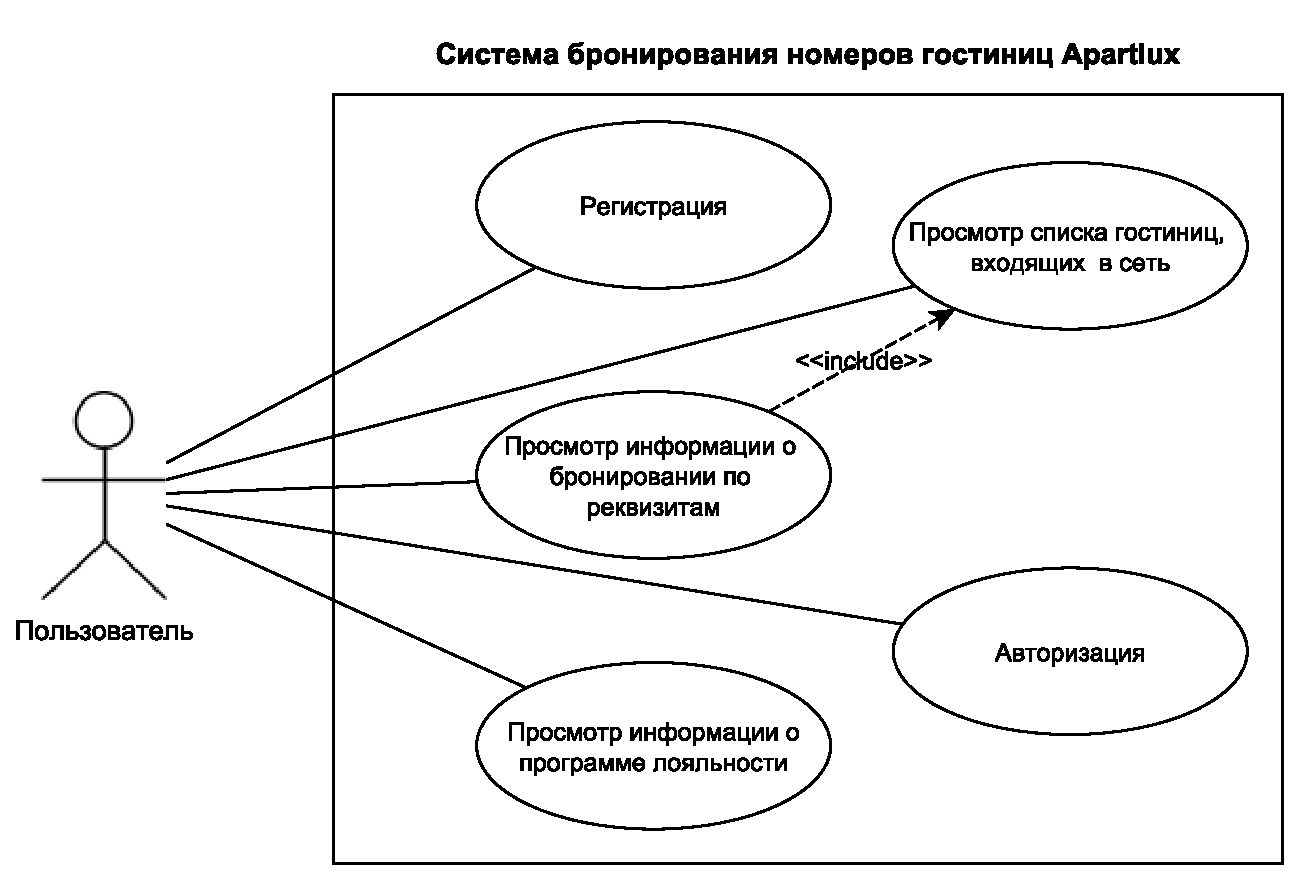
\includegraphics[scale = 0.6]{img/use-case/user.pdf}}
		\caption{Диаграмма прецедентов с точки зрения пользователя.}
		\label{fig:use-case-user}
	\end{center}
\end{figure}

\pagebreak

\begin{longtable}{| p{6cm} | p{10cm} |}
	\caption{Спецификация сценария регистрации}
	\label{tbl:scenario-1} \\
	\hline
	
	\multicolumn{2}{|c|}{\textbf{Нормальный ход сценария}} \\
	\hline
	
	\textbf{Действия пользователя} & \textbf{Отклик системы} \\
	\hline
	\endfirsthead
	
	\hline
	\textbf{Действия пользователя} & \textbf{Отклик системы} \\
	\hline
	\endhead
	
	\hline
	\multicolumn{2}{c}{\textit{Продолжение на следующей странице}}
	\endfoot
	\hline
	\endlastfoot
	
	Регистрация
	&
	Система предоставляет пользователю форму для регистрации, в которой нужно заполнить ФИО, дату рождения, логин, пароль, номер телефона, электронную почту \\
	\hline
	
	Пользователь заполняет форму и даёт согласие на обработку данных
	&
	Данные пользователя регистрируются в системе \\
	\hline
	
	\multicolumn{2}{|c|}{\textbf{Альтернативный ход сценария}} \\
	\hline
	
	Регистрация
	&
	Система предоставляет пользователю форму для регистрации, в которой нужно заполнить ФИО, дату рождения, логин, пароль, номер телефона, электронную почту \\
	\hline
	
	Пользователь не заполняет форму или не даёт согласие на обработку данных
	&
	Пользователь не заносится в клиентскую базу данных
\end{longtable}

\begin{figure}[h]
	\begin{center}
		{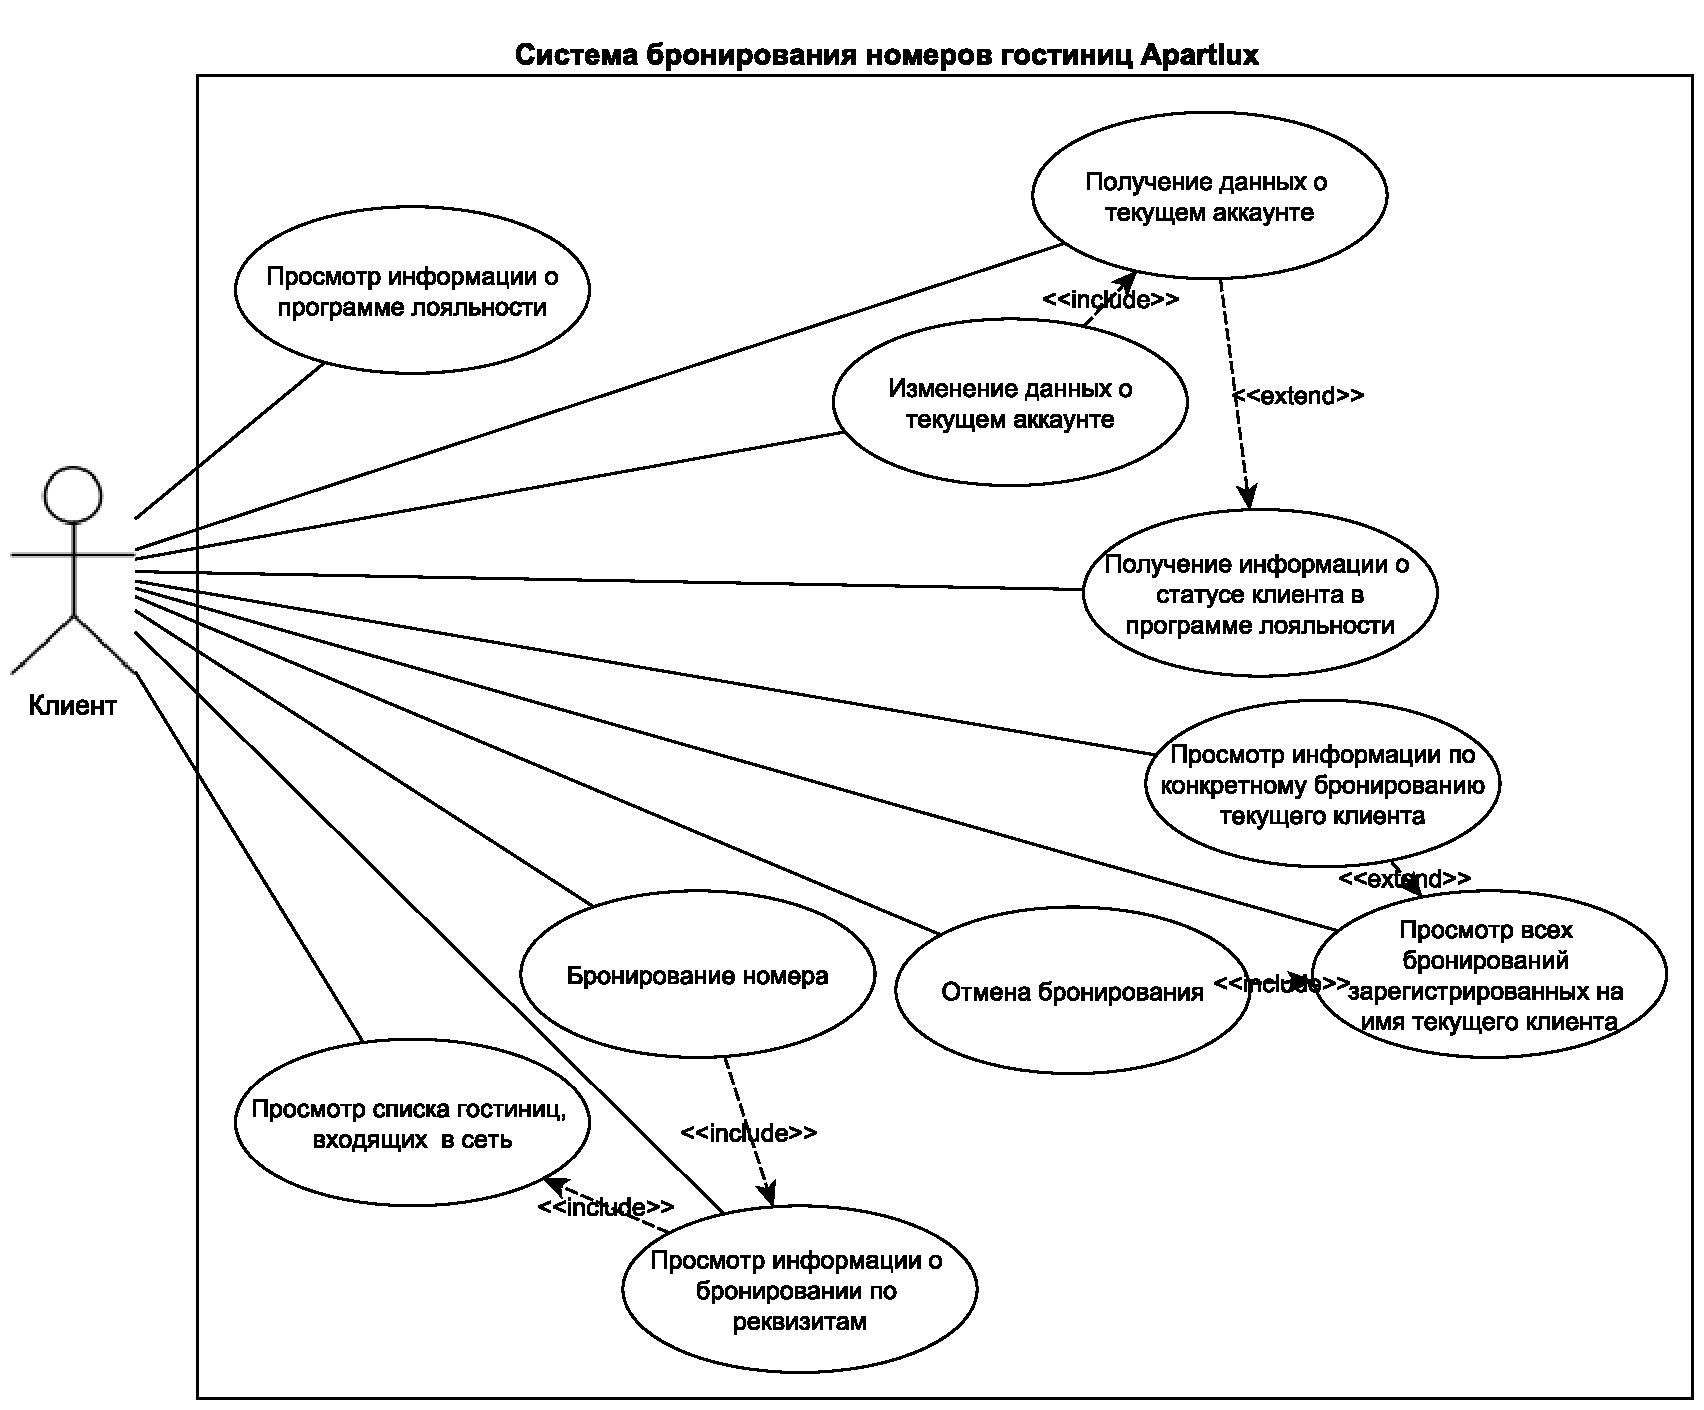
\includegraphics[scale = 0.56]{img/use-case/client.pdf}}
		\caption{Диаграмма прецедентов с точки зрения клиента.}
		\label{fig:use-case-client}
	\end{center}
\end{figure}

\begin{longtable}{| p{6cm} | p{10cm} |}
	\caption{Спецификация сценария бронирования}
	\label{tbl:scenario-2} \\
	\hline
	
	\multicolumn{2}{|c|}{\textbf{Нормальный ход сценария}} \\
	\hline
	
	\textbf{Действия клиента} & \textbf{Отклик системы} \\
	\hline
	\endfirsthead
	
	\hline
	\textbf{Действия клиента} & \textbf{Отклик системы} \\
	\hline
	\endhead
	
	\hline
	\multicolumn{2}{c}{\textit{Продолжение на следующей странице}}
	\endfoot
	\hline
	\endlastfoot
	
	Просмотр списка гостиниц, предварительно отфильтрованных по выставленным пользователем параметрам
	&
	Система предоставляет клиенту список гостиниц, которые входят в состав сети Apartlux и предоставляющих свободные для бронирования номера \\
	\hline
	
	Просмотр информации о возможном бронировании по заданным реквизитам (дата, цена, количество мест и т.д.)
	&
	Система предоставляет клиенту ранжированный список номеров, наиболее подходящих под параметры фильтрации, указанные клиентом \\
	\hline
	
	Бронирование
	&
	Система перенаправляет клиенту на страницу подтверждения по коду из смс, после успешной операции фиксирует выбранный номер за клиентом \\
	\hline
	
	\multicolumn{2}{|c|}{\textbf{Альтернативный ход сценария}} \\
	\hline
	
	Просмотр списка гостиниц, предварительно отфильтрованных по выставленным пользователем параметрам
	&
	Система предоставляет клиенту список гостиниц, которые входят в состав сети Apartlux и предоставляющих свободные для бронирования номера \\
	\hline
	
	Клиент не выбирает ни одну гостиницу из предоставленных
	&
	Система отправляет письмо-напоминание на почту клиента, содержащее список предлагаемых гостиниц
	\\
	\hline
	
	\multicolumn{2}{|c|}{\textbf{Альтернативный ход сценария}} \\
	\hline
	
	Система не смогла подобрать ни одной гостиницы, которая бы подходила под желания пользователя
	&
	Система выводит сообщение об отсутствии позиций, точно подходящих под описание, а также предоставляет список гостиниц, которые частично подходят под реквизиты
	\\
	\hline
	
	\multicolumn{2}{|c|}{\textbf{Альтернативный ход сценария}} \\
	\hline
	
	Просмотр списка гостиниц, предварительно отфильтрованных по выставленным пользователем параметрам
	&
	Система предоставляет клиенту список гостиниц, которые входят в состав сети Apartlux и предоставляющих свободные для бронирования номера \\
	\hline
	
	Просмотр информации о возможном бронировании по заданным реквизитам (дата, цена, количество мест и т.д.)
	&
	Система предоставляет клиенту ранжированный список номеров, наиболее подходящих под параметры фильтрации, указанные клиентом \\
	\hline
	
	Клиент не выбирает ни одного номера и завершает работу с системой
	&
	Система отправляет письмо-напоминание на почту клиента, содержащее список предлагаемых номеров
	\\
	\hline
	
	\multicolumn{2}{|c|}{\textbf{Альтернативный ход сценария}} \\
	\hline
	
	Просмотр списка гостиниц, предварительно отфильтрованных по выставленным пользователем параметрам
	&
	Система предоставляет клиенту список гостиниц, которые входят в состав сети Apartlux и предоставляющих свободные для бронирования номера \\
	\hline
	
	Система не смогла подобрать ни одного номера, который бы подходил под желания клиента  (дата, цена, количество мест и т.д.)
	&
	Система предоставляет клиенту ранжированный список номеров, наиболее подходящих под параметры фильтрации, указанные клиентом \\
	\hline
	
	
	\multicolumn{2}{|c|}{\textbf{Альтернативный ход сценария}} \\
	\hline
	
	Просмотр списка гостиниц, входящих в сеть
	&
	Система предоставляет клиент список гостиниц, которые входят в состав сети Apartlux и предоставляющих свободные для бронирования номера \\
	\hline
	
	Просмотр информации о возможном бронировании по заданным реквизитам (дата, цена, количество мест и т.д.)
	&
	Система предоставляет клиент ранжированный список номеров, наиболее подходящих под параметры фильтрации, указанные клиентом \\
	\hline
	
	Бронирование (операции подтверждения по смс завершилась с ошибкой)
	&
	Система выводит сообщение об ошибке на экран, из-за проблем с операцией клиенту предлагается повторить попытку, номер на клиента не регистрируется
\end{longtable}

\begin{figure}[h!]
	\begin{center}
		{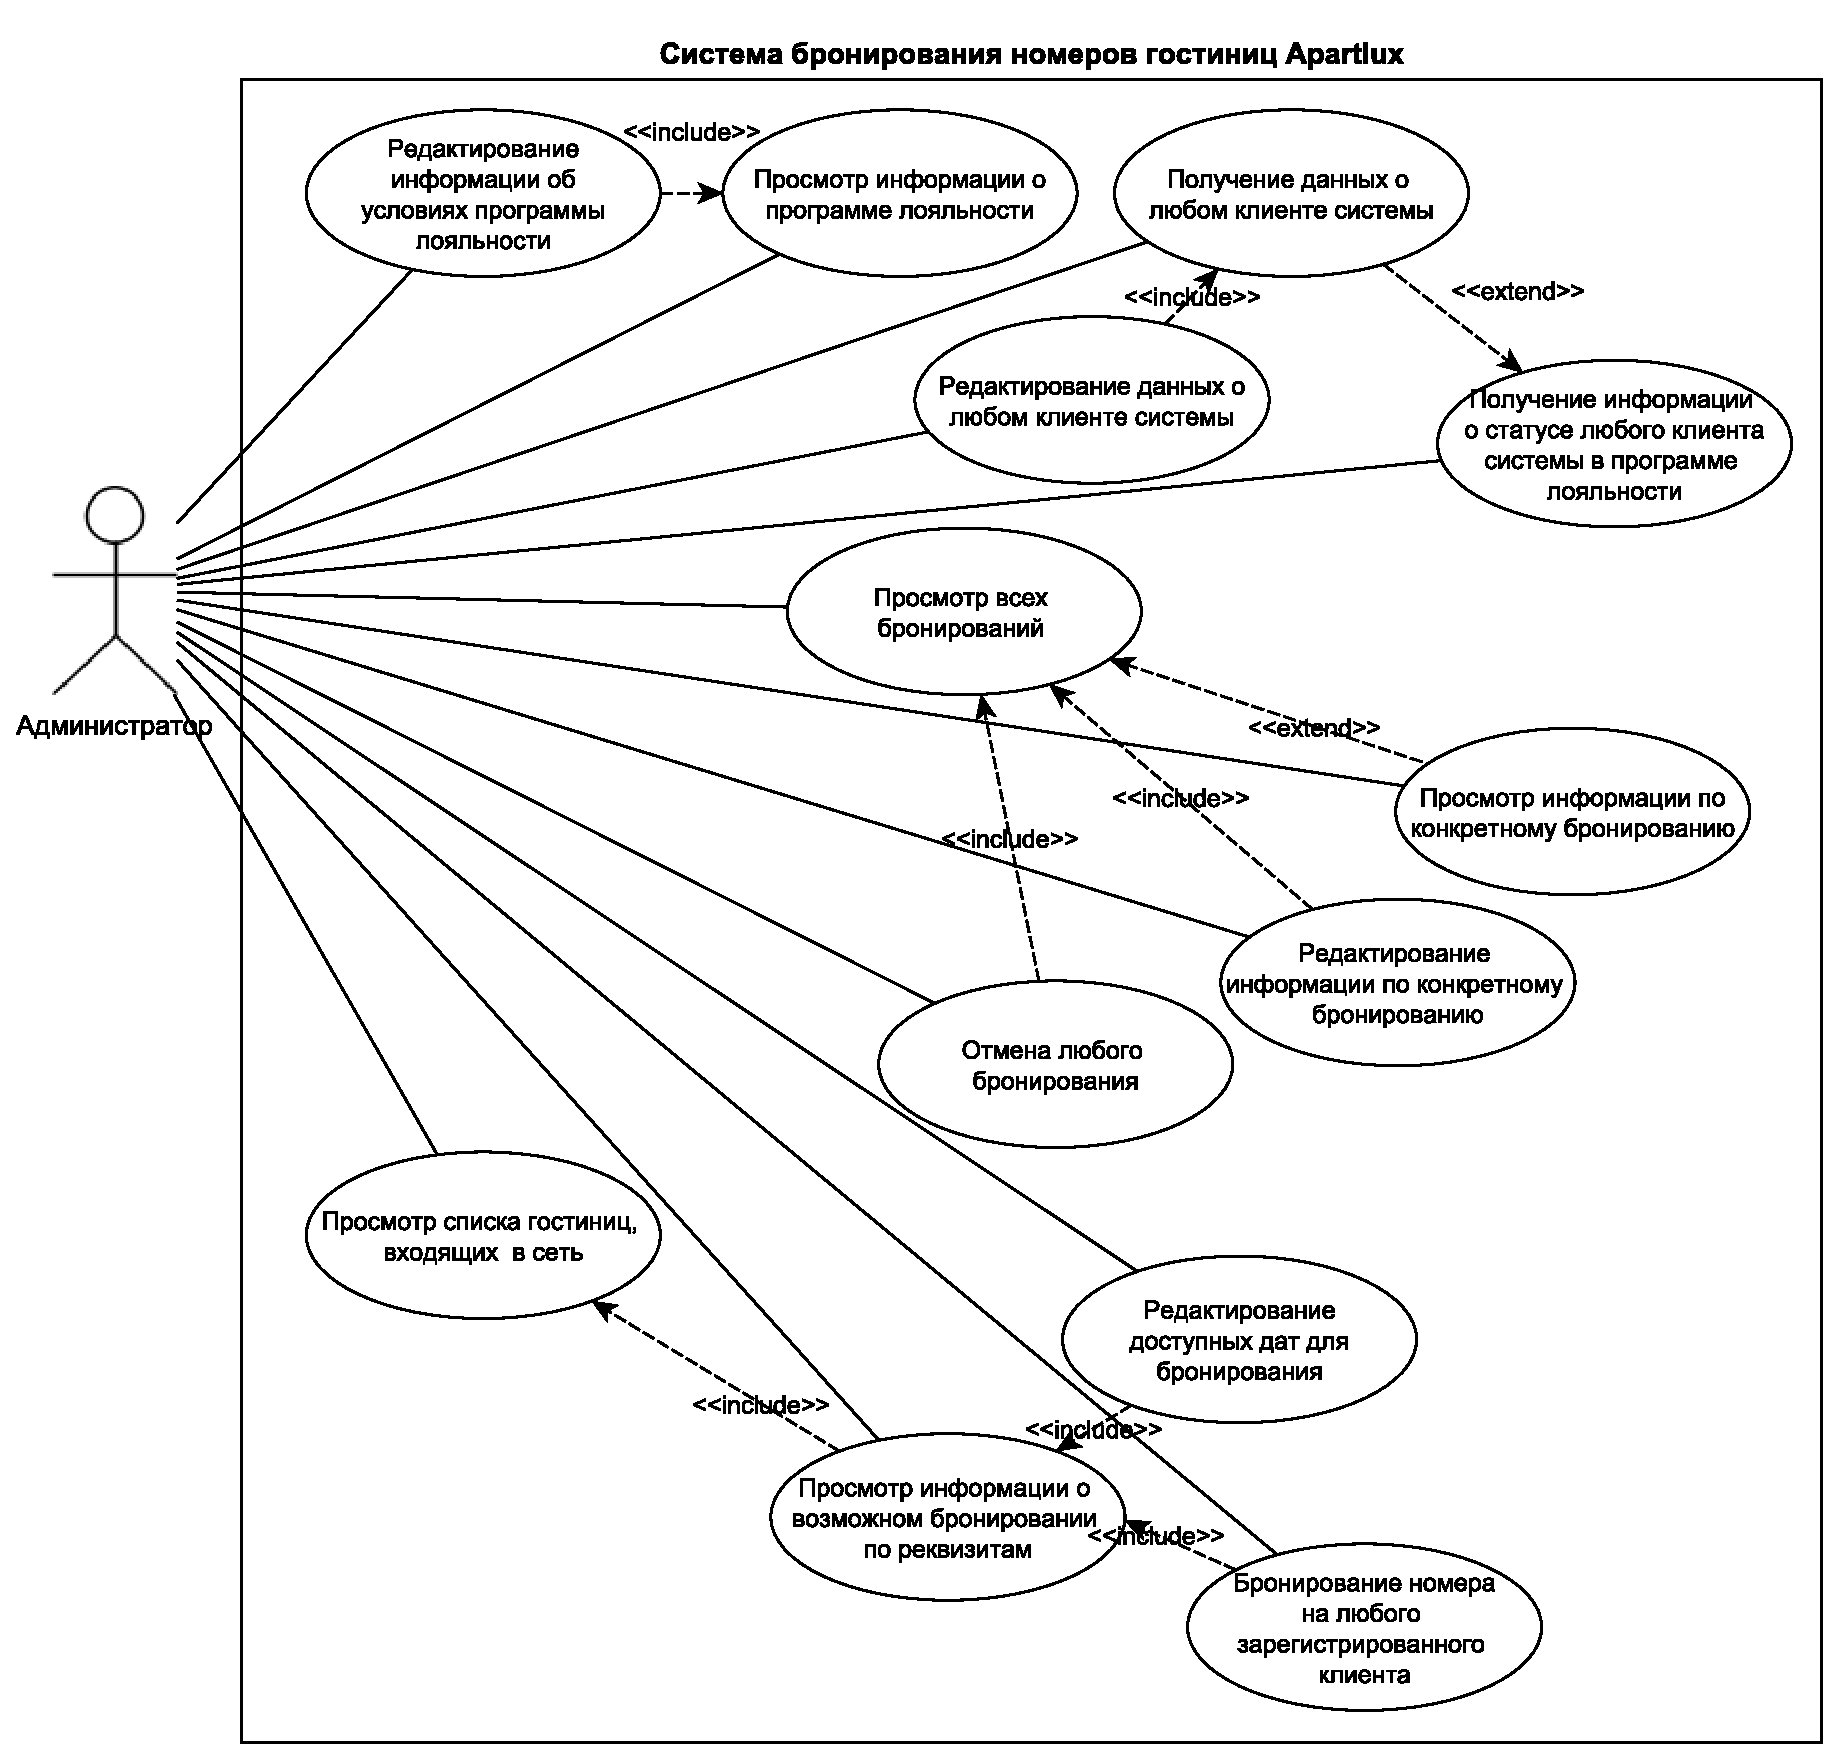
\includegraphics[scale = 0.54]{img/use-case/admin.pdf}}
		\caption{Диаграмма прецедентов с точки зрения администратора.}
		\label{fig:use-case-admin}
	\end{center}
\end{figure}

\pagebreak

\section*{Спецификация классов}
На рисунке \ref{fig:diag-classes} представлена диаграмма классов для разработки микросервиса бронирования.

\begin{figure}[h!]
	\begin{center}
		{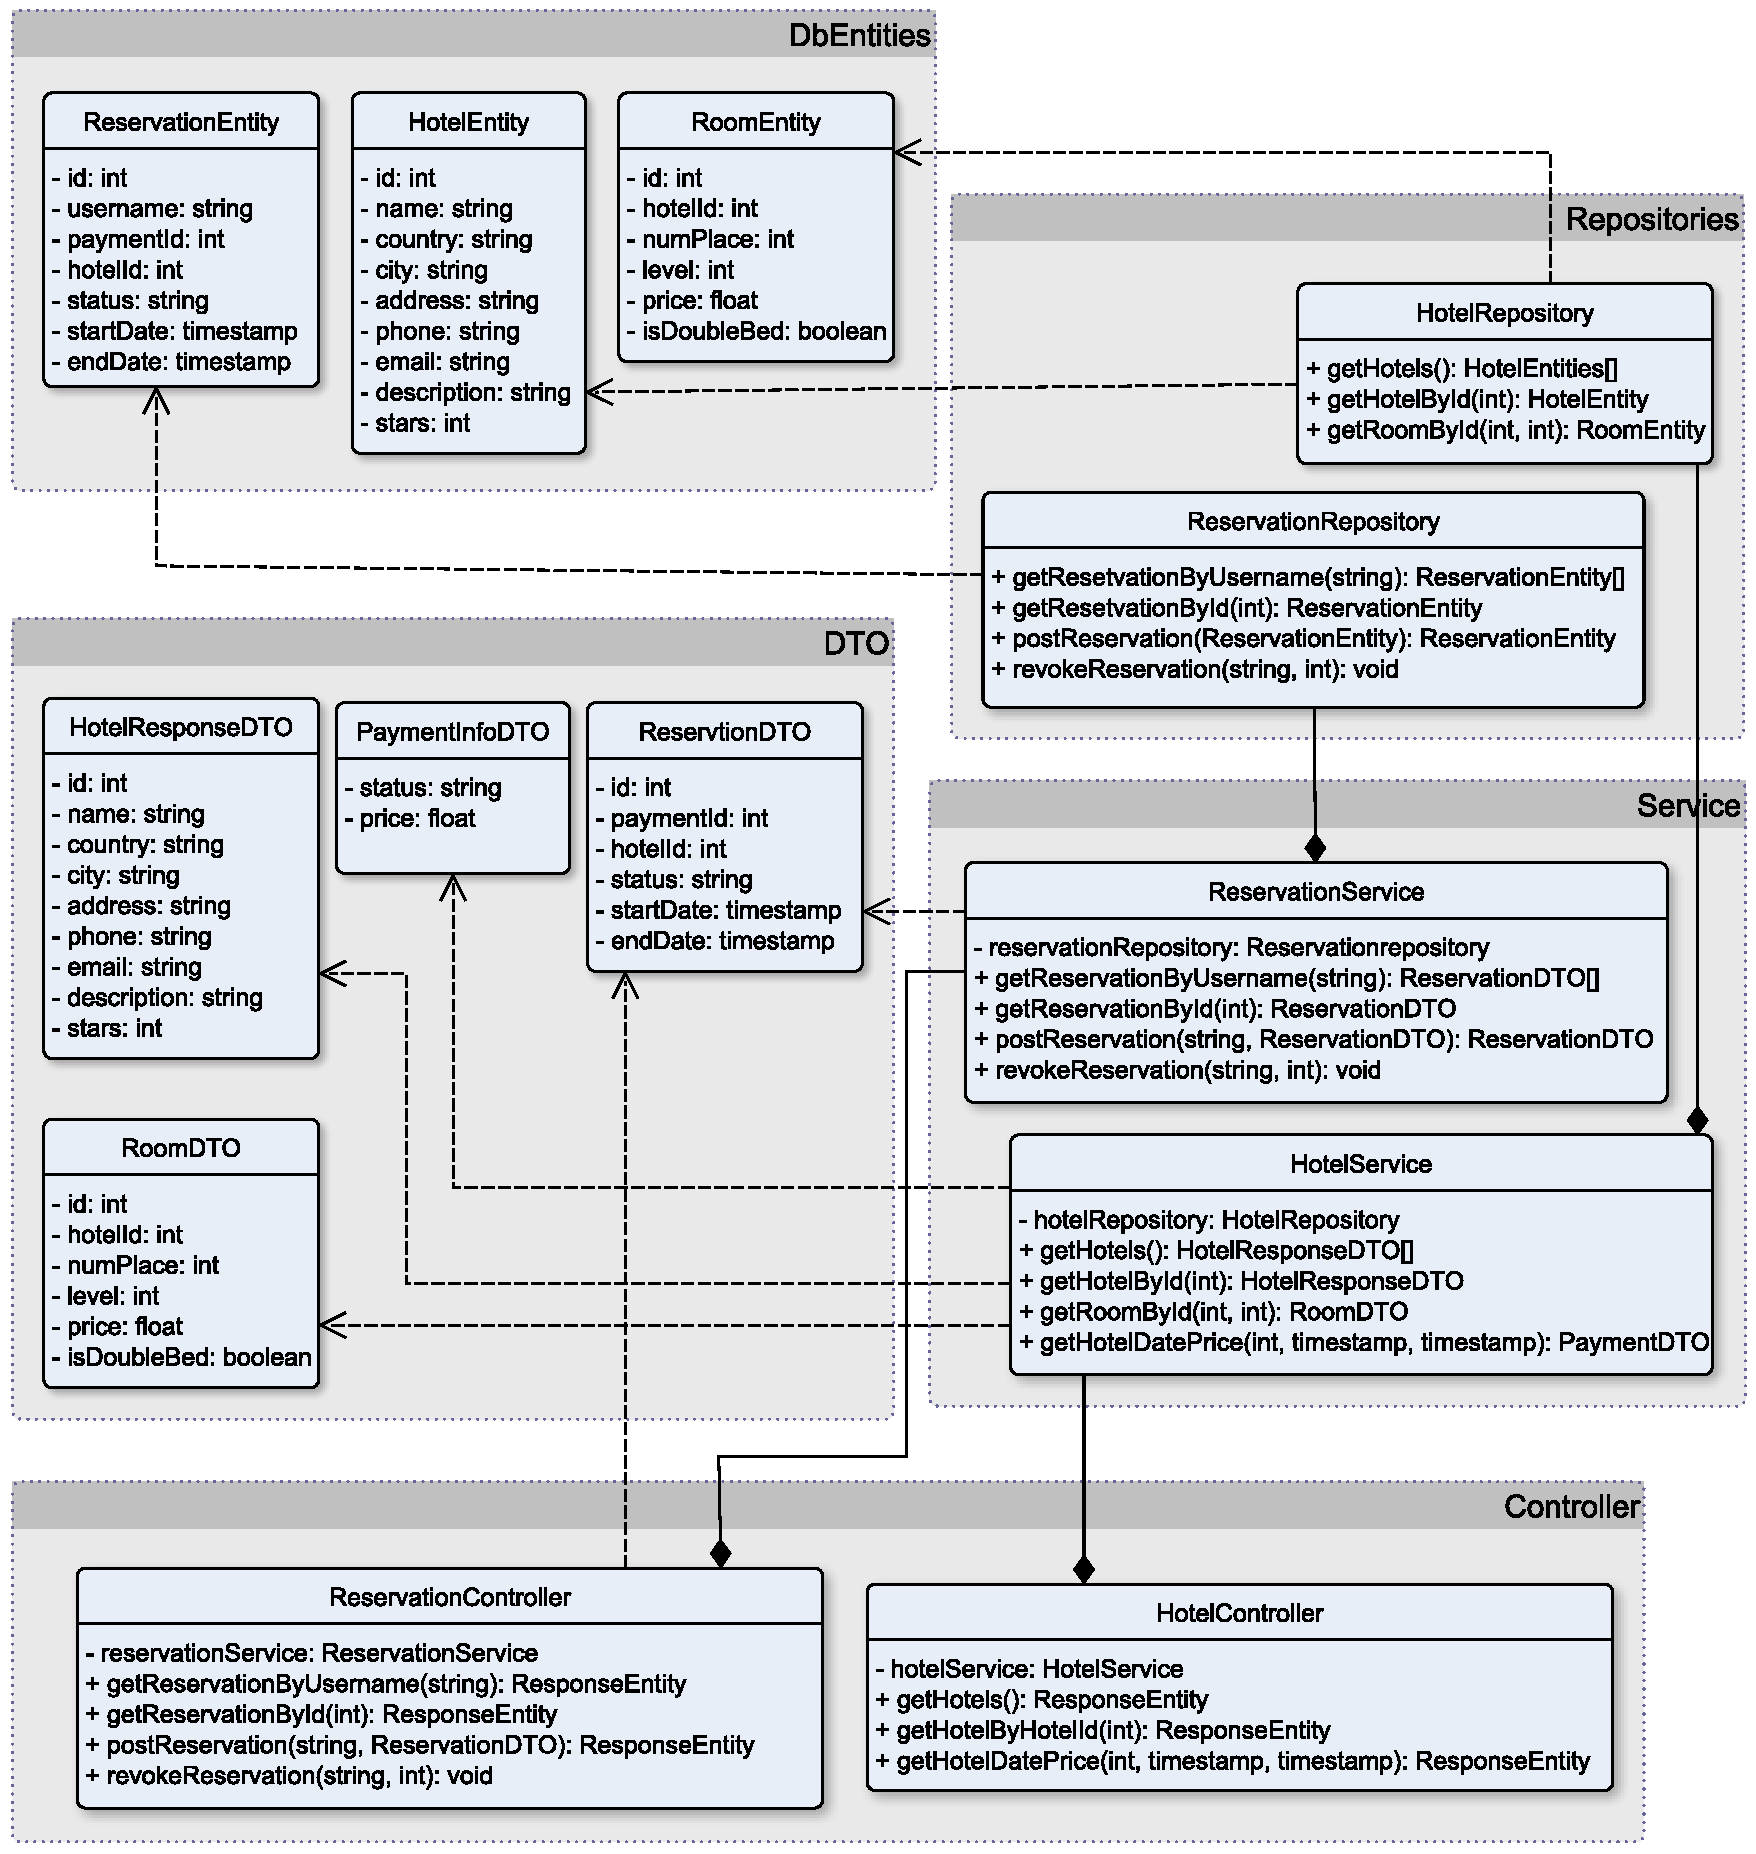
\includegraphics[scale = 0.58]{img/diag_classes/classes.pdf}}
		\caption{Диаграмма классов.}
		\label{fig:diag-classes}
	\end{center}
\end{figure} 

Классы ReservationEntity, HotelEntity, RoomEntity представляют легковесные объекты бизнес-логики, ассоциированные с соответствующими сущностями базы данных. Атрибуты указанных классов представлены в таблицах \ref{tbl:hotel-entity}-\ref{tbl:reservation-entity}.

\begin{longtable}{| p{3cm} | p{5cm} | p{8cm} |}
	\caption{Атрибуты класса HotelEntity}
	\label{tbl:hotel-entity} \\
	\hline
	
	\multicolumn{3}{|c|}{\textbf{Атрибуты}} \\
	\hline
	
	\textbf{Имя} & \textbf{Тип} & \textbf{Описание} \\
	\hline
	\endfirsthead
	
	\hline
	\textbf{Имя} & \textbf{Тип} & \textbf{Описание} \\
	\hline
	\endhead
	
	\hline
	\multicolumn{3}{c}{\textit{Продолжение на следующей странице}}
	\endfoot
	\hline
	\endlastfoot
	
	id
	&
	private: int
	&
	идентификатор \\
	\hline
	
	name
	&
	private: string
	&
	название \\
	\hline
	
	country
	&
	private: string
	&
	страна \\
	\hline
	
	city
	&
	private: string
	&
	город \\
	\hline
	
	address
	&
	private: string
	&
	адрес \\
	\hline
	
	phone
	&
	private: string
	&
	контактный телефон \\
	\hline
	
	email
	&
	private: string
	&
	электронная почта \\
	\hline
	
	description
	&
	private: string
	&
	описание \\
	\hline
	
	stars
	&
	private: int
	&
	количество звёзд \\
\end{longtable}

\begin{longtable}{| p{3cm} | p{5cm} | p{8cm} |}
	\caption{Атрибуты класса RoomEntity}
	\label{tbl:room-entity} \\
	\hline
	
	\multicolumn{3}{|c|}{\textbf{Атрибуты}} \\
	\hline
	
	\textbf{Имя} & \textbf{Тип} & \textbf{Описание} \\
	\hline
	\endfirsthead
	
	\hline
	\textbf{Имя} & \textbf{Тип} & \textbf{Описание} \\
	\hline
	\endhead
	
	\hline
	\multicolumn{3}{c}{\textit{Продолжение на следующей странице}}
	\endfoot
	\hline
	\endlastfoot
	
	id
	&
	private: int
	&
	идентификатор \\
	\hline
	
	hotelId
	&
	private: int
	&
	идентификатор гостиницы \\
	\hline
	
	numPlace
	&
	private: int
	&
	число мест \\
	\hline
	
	level
	&
	private: int
	&
	этаж \\
	\hline
	
	price
	&
	private: float
	&
	стоимость \\
	\hline
	
	isDoubleBed
	&
	private: boolean
	&
	признак наличия двуспальной кровати \\
\end{longtable}

\begin{longtable}{| p{3cm} | p{5cm} | p{8cm} |}
	\caption{Атрибуты класса ReservationEntity}
	\label{tbl:reservation-entity} \\
	\hline
	
	\multicolumn{3}{|c|}{\textbf{Атрибуты}} \\
	\hline
	
	\textbf{Имя} & \textbf{Тип} & \textbf{Описание} \\
	\hline
	\endfirsthead
	
	\hline
	\textbf{Имя} & \textbf{Тип} & \textbf{Описание} \\
	\hline
	\endhead
	
	\hline
	\multicolumn{3}{c}{\textit{Продолжение на следующей странице}}
	\endfoot
	\hline
	\endlastfoot
	
	id
	&
	private: int
	&
	идентификатор \\
	\hline
	
	username
	&
	private: string
	&
	логин клиента \\
	\hline
	
	paymentId
	&
	private: int
	&
	идентификатор платёжной операции \\
	\hline
	
	hotelId
	&
	private: int
	&
	идентификатор гостиницы \\
	\hline
	
	status
	&
	private: string
	&
	статус \\
	\hline
	
	startDate
	&
	private: timestamp
	&
	дата въезда \\
	\hline
	 
	endDate
	&
	private: timestamp
	&
	дата выезда \\
\end{longtable}

Классы ReservationDTO, HotelResponseDTO, RoomDTO, PaymentInfoDTO представляют объекты для передачи данных между классами бизнес-логики. Атрибутивный состав ReservationDTO, HotelResponseDTO, RoomDTO аналогичен составу ассоциированных с ними сущностей базы данных.  Атрибуты вспомогательного класса PaymentInfoDTO представлены в таблице \ref{tbl:paymentInfo-dto}.

\begin{longtable}{| p{3cm} | p{5cm} | p{8cm} |}
	\caption{Атрибуты класса PaymentInfoDTO}
	\label{tbl:paymentInfo-dto} \\
	\hline
	
	\multicolumn{3}{|c|}{\textbf{Атрибуты}} \\
	\hline
	
	\textbf{Имя} & \textbf{Тип} & \textbf{Описание} \\
	\hline
	\endfirsthead
	
	\hline
	\textbf{Имя} & \textbf{Тип} & \textbf{Описание} \\
	\hline
	\endhead
	
	\hline
	\multicolumn{3}{c}{\textit{Продолжение на следующей странице}}
	\endfoot
	\hline
	\endlastfoot
	
	status
	&
	private: string
	&
	статус операции \\
	\hline
	
	price
	&
	private: float
	&
	стоимость \\
\end{longtable}

Классы HotelRepository и ReservationRepository отвечают за взаимодействие микросервиса с базой данных. Методы каждого приведены в таблицах \ref{tbl:hotelrepository}-\ref{tbl:reservationrepository}.

\begin{longtable}{| p{8cm} | p{8cm} |}
	\caption{Атрибуты класса HotelRepository}
	\label{tbl:hotelrepository} \\
	\hline
	
	\multicolumn{2}{|c|}{\textbf{Методы}} \\
	\hline
	
	\textbf{Название} & \textbf{Описание} \\
	\hline
	\endfirsthead
	
	\hline
	\textbf{Название} & \textbf{Описание} \\
	\hline
	\endhead
	
	\hline
	\multicolumn{2}{c}{\textit{Продолжение на следующей странице}}
	\endfoot
	\hline
	\endlastfoot
	
	getHotelById(int): HotelEntity
	&
	param: id [int - in] - идентификатор \newline
	\textit{получение информации о гостинице по её идентификатору }\\
	\hline
	
	getRoomById(int, int): RoomEntity
	&
	param: idHotel [int - in] - идентификатор гостинцы \newline
	param: idRoom [int - in] - идентификатор номера \newline
	\textit{получение информации о номере по идентификаторам гостиницы и номера }\\
\end{longtable}

\begin{longtable}{| p{8cm} | p{8cm} |}
	\caption{Атрибуты класса ReservationRepository}
	\label{tbl:reservationrepository} \\
	\hline
	
	\multicolumn{2}{|c|}{\textbf{Методы}} \\
	\hline
	
	\textbf{Название} & \textbf{Описание} \\
	\hline
	\endfirsthead
	
	\hline
	\textbf{Название} & \textbf{Описание} \\
	\hline
	\endhead
	
	\hline
	\multicolumn{2}{c}{\textit{Продолжение на следующей странице}}
	\endfoot
	\hline
	\endlastfoot
	
	getReservationByUsername(string): ReservationEntity[]
	&
	param: [string - in] - логин клиента \newline
	\textit{получение информации о бронированиях по логину клиента }\\
	\hline
	
	getReservationById(int): ReservationEntity
	&
	param: [int - in] - идентификатор бронирования \newline
	\textit{получение информации о бронировании по его идентификатору }\\
	\hline
	
	postReservation(ReservationEntity): ReservationEntity
	&
	param: [ReservationEntity - in] - бронирование \newline
	\textit{создание записи о бронировании} \\
	\hline
	
	revokeReservation(string, int): void
	&
	param: [string - in] - логин клиента \newline
	param: [int - in] - идентификатор бронирования \newline
	\textit{отмена бронирования }\\
\end{longtable}

Классы ReservationService и HotelService реализуют основную бизнес-логику микросервиса, преобразование данных и передачу их на последующий слой, непосредственно связанный с базой данных, поэтому предоставляемые ими методы схожи с методами классов ReservationRepository и HotelRepository.

На рисунке \ref{fig:schema-reservation} представлена диаграмма деятельности в режиме <<Бронирование>> для клиента.

\begin{figure}[h!]
	\begin{center}
		{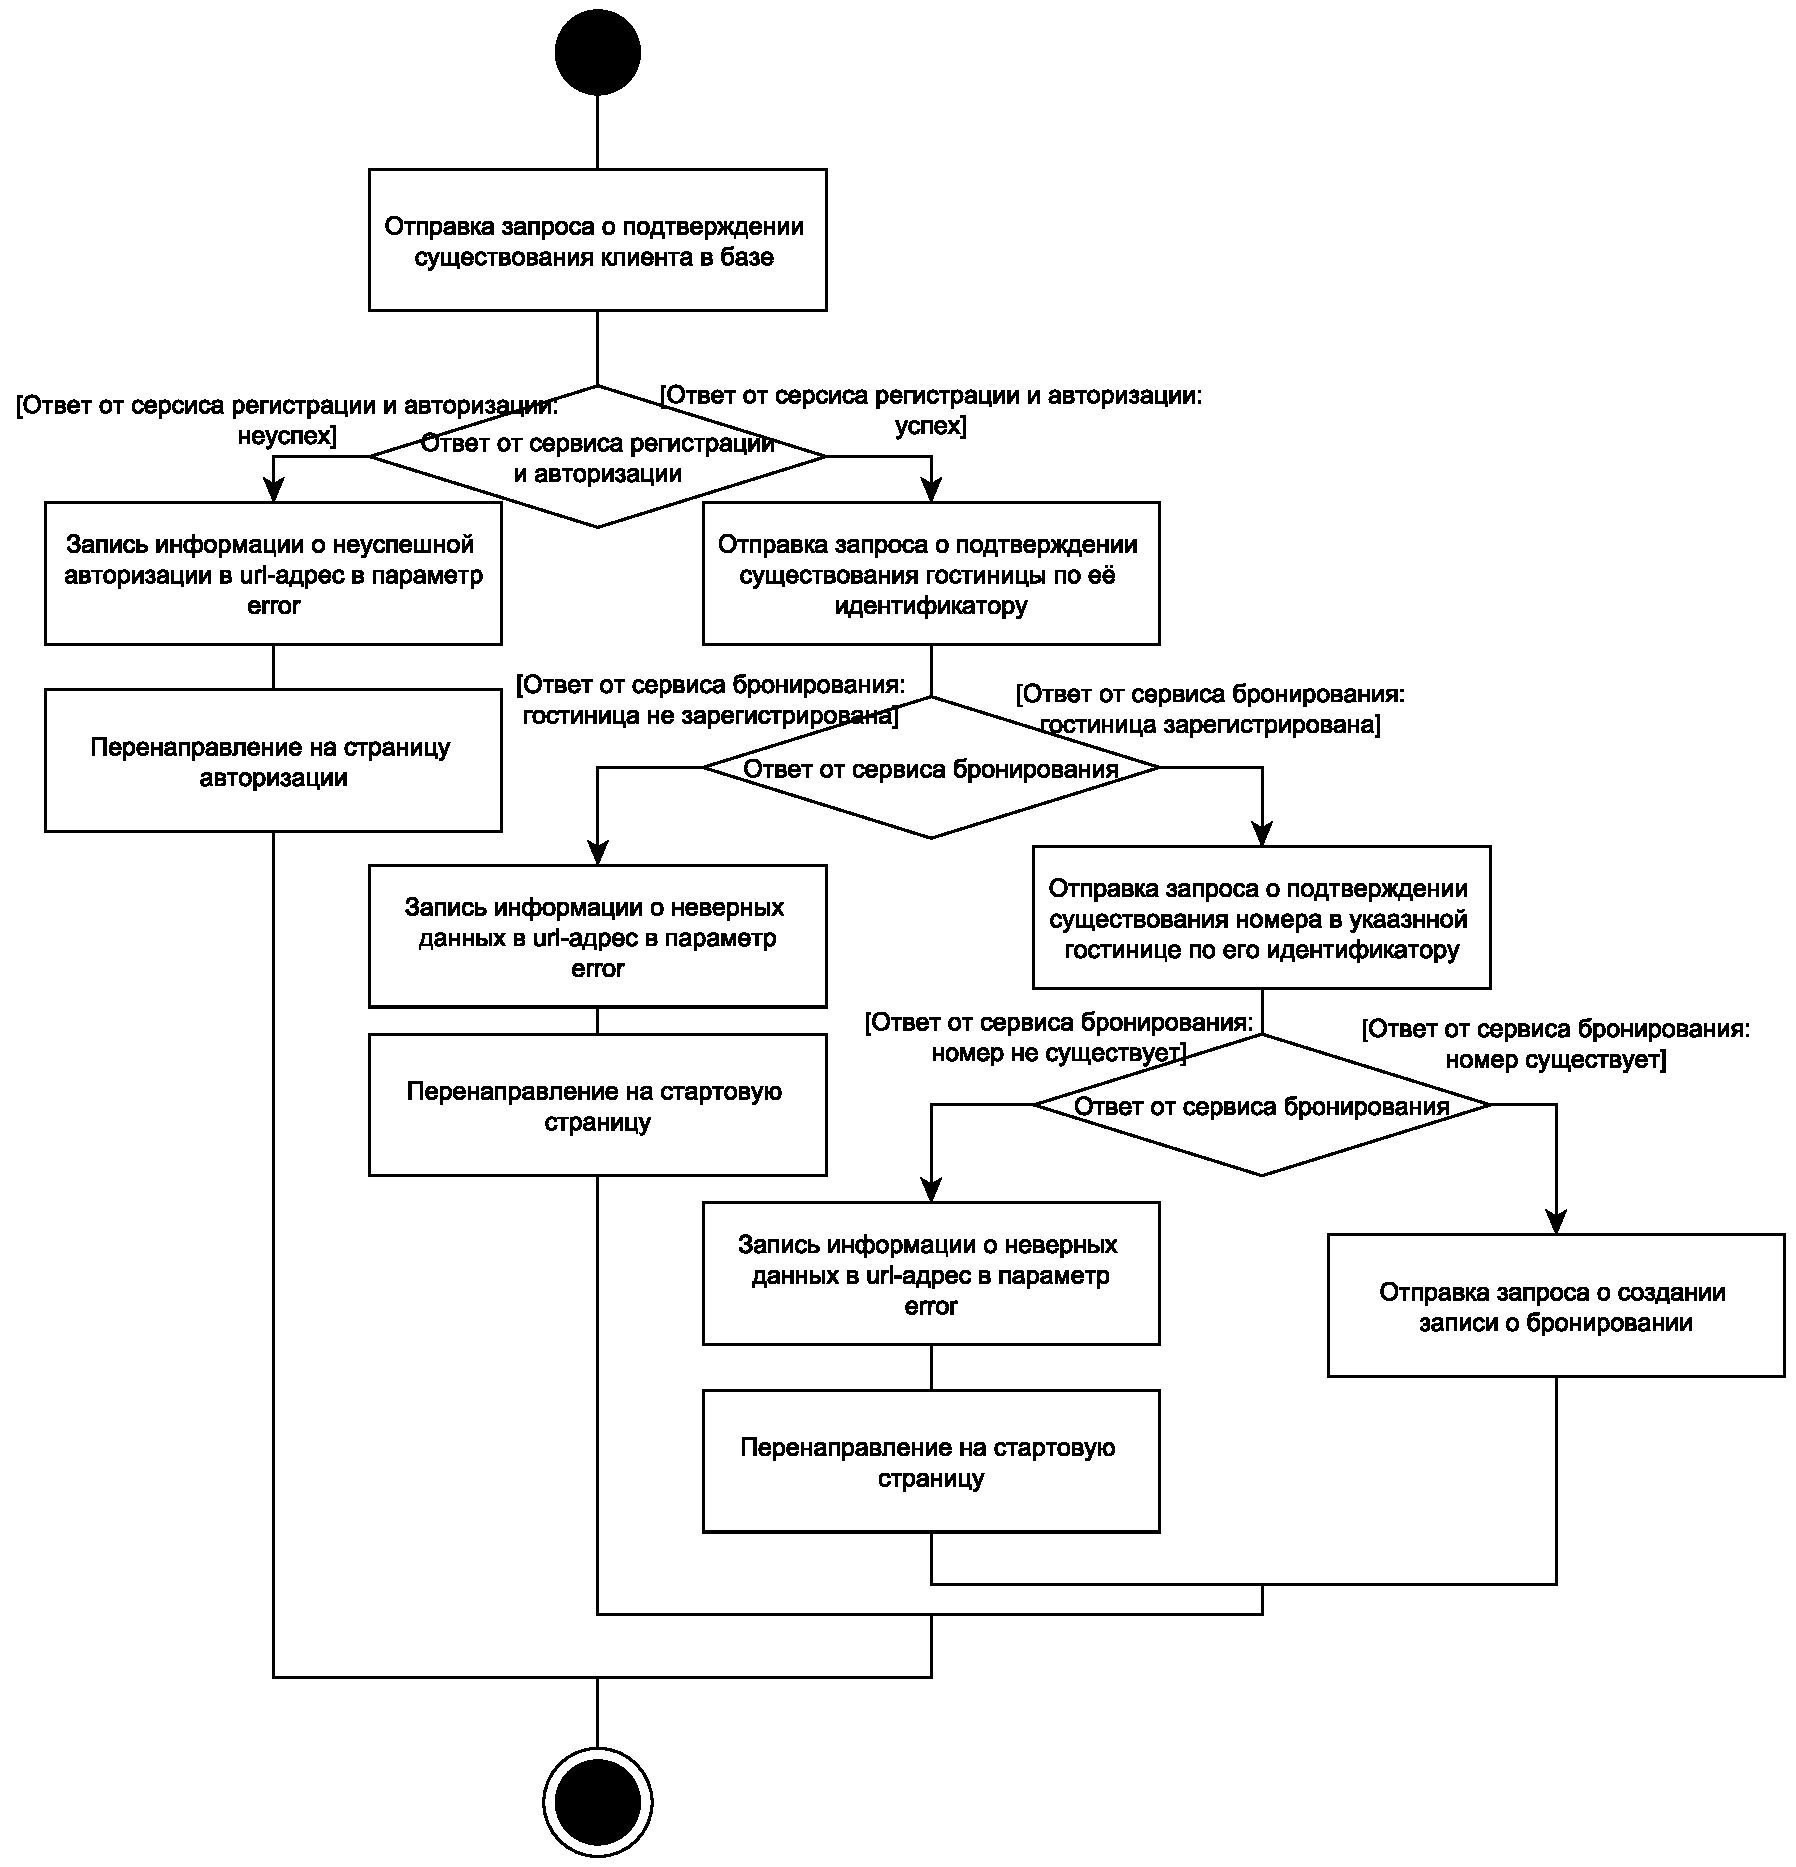
\includegraphics[scale = 0.58]{img/schemas/schema-1.pdf}}
		\caption{Диаграмма деятельности в режиме <<Бронирование>> для клиента.}
		\label{fig:schema-reservation}
	\end{center}
\end{figure}

\pagebreak

На рисунке \ref{fig:flow-level1} представлена наиболее важная для системы динамическая модель, представленная в виде диаграммы деятельности.

\begin{figure}[h!]
	\begin{center}
		{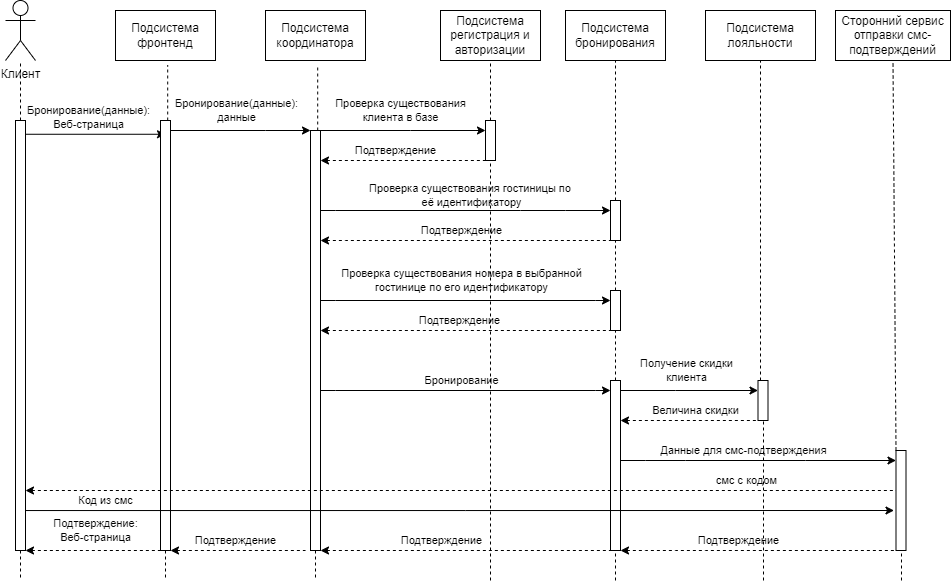
\includegraphics[angle = 90, scale = 0.63]{img/flow/diag_general.png}}
		\caption{Диаграмма последовательности действий при бронировании номера клиентом: концептуальный уровень.}
		\label{fig:flow-level1}
	\end{center}
\end{figure}

\pagebreak

В системе предполагается распределенное хранение данных. Диаграмма потоков данных, представленная на рисунке \ref{fig:data_flow}, позволяет описать распределение сохраняемой информации в хранилищах данных. Каждое хранилище данных будет реализовано в виде базы данных.

\begin{figure}[h!]
	\begin{center}
		{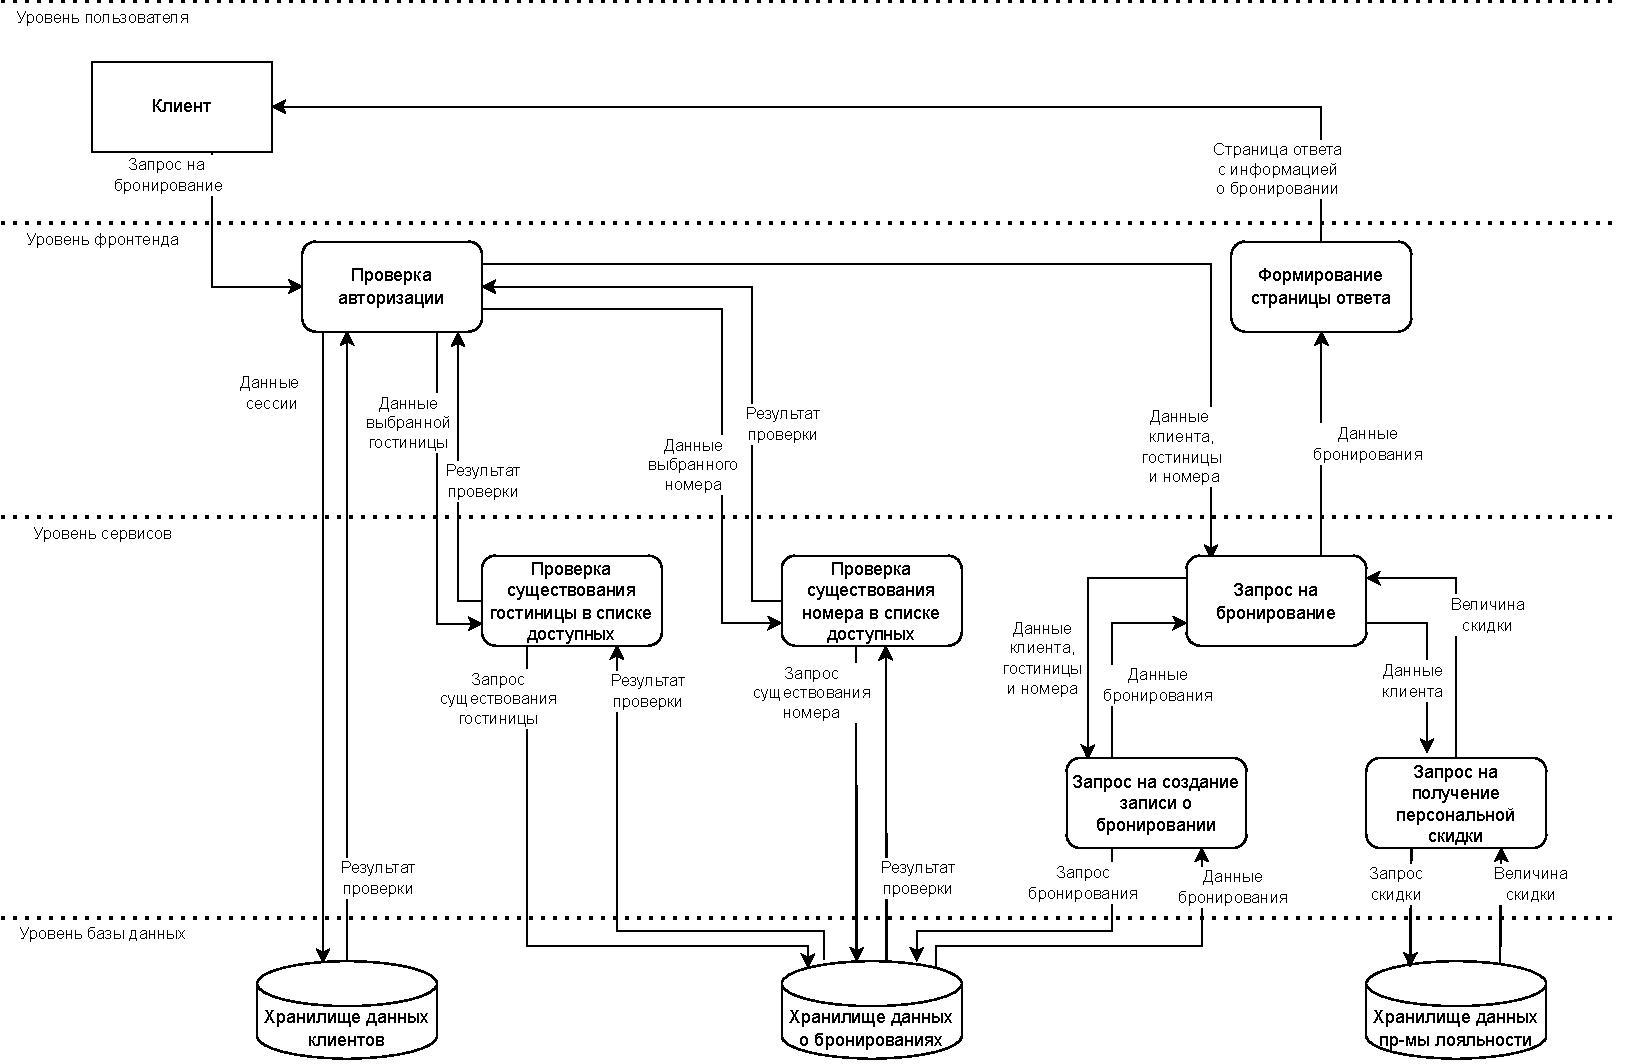
\includegraphics[angle = 90, scale = 0.725]{img/flow/data_flow.pdf}}
		\caption{Диаграмма потоков данных при бронировании.}
		\label{fig:data_flow}
	\end{center}
\end{figure} 

\pagebreak

\section*{Высокоуровневый дизайн пользовательского интерфейса}
Пользовательский интерфейс в разрабатываемой системе представляет собой web-интерфейс, доступ к которому осуществляется через браузер (тонкий клиент).

Страница системы состоит из «шапки», основной части и футера.  «Шапка» —  это  верхняя  часть  страницы,  в  которой находятся логотип и верхнее меню со ссылками на основные разделы портала. Футер — это нижняя часть страницы, в которой обычно размещают ссылки  на  редко  посещаемые,  но  необходимые  страницы,  например, страницы с пользовательским соглашением.

Обобщенно структуру страниц системы можно представить следующим образом:
\begin{itemize}
	\item главная страница с перечнем наиболее популярных гостиниц сети;
	
	\item страница авторизации;
		
	\item форма регистрации;
	
	\item страница с информацией о гостинице и списком доступных для бронирования номеров;
	
	\item страница с детальной информацией по конкретному номеру;
	
	\item страница личного кабинета клиента системы;
	
	\item о нас
	\begin{itemize}
		\item контакты;
		
		\item новости;
		
		\item нормативные документы;
		
		\item правила организации.
	\end{itemize}
\end{itemize}

Ниже приведены такие формы системы, как страницы регистрации нового клиента и главная старница со списком гостиниц, в который есть свободные для бронирования номера. На рисунке \ref{fig:ui-reg} представлена форма регистрации, на которой пользователю нужно ввести личные данные: ФИО, дата рождения, телефон, электронная почта, также придумать логин и пароль. 

\begin{figure}[h]
	\begin{center}
		{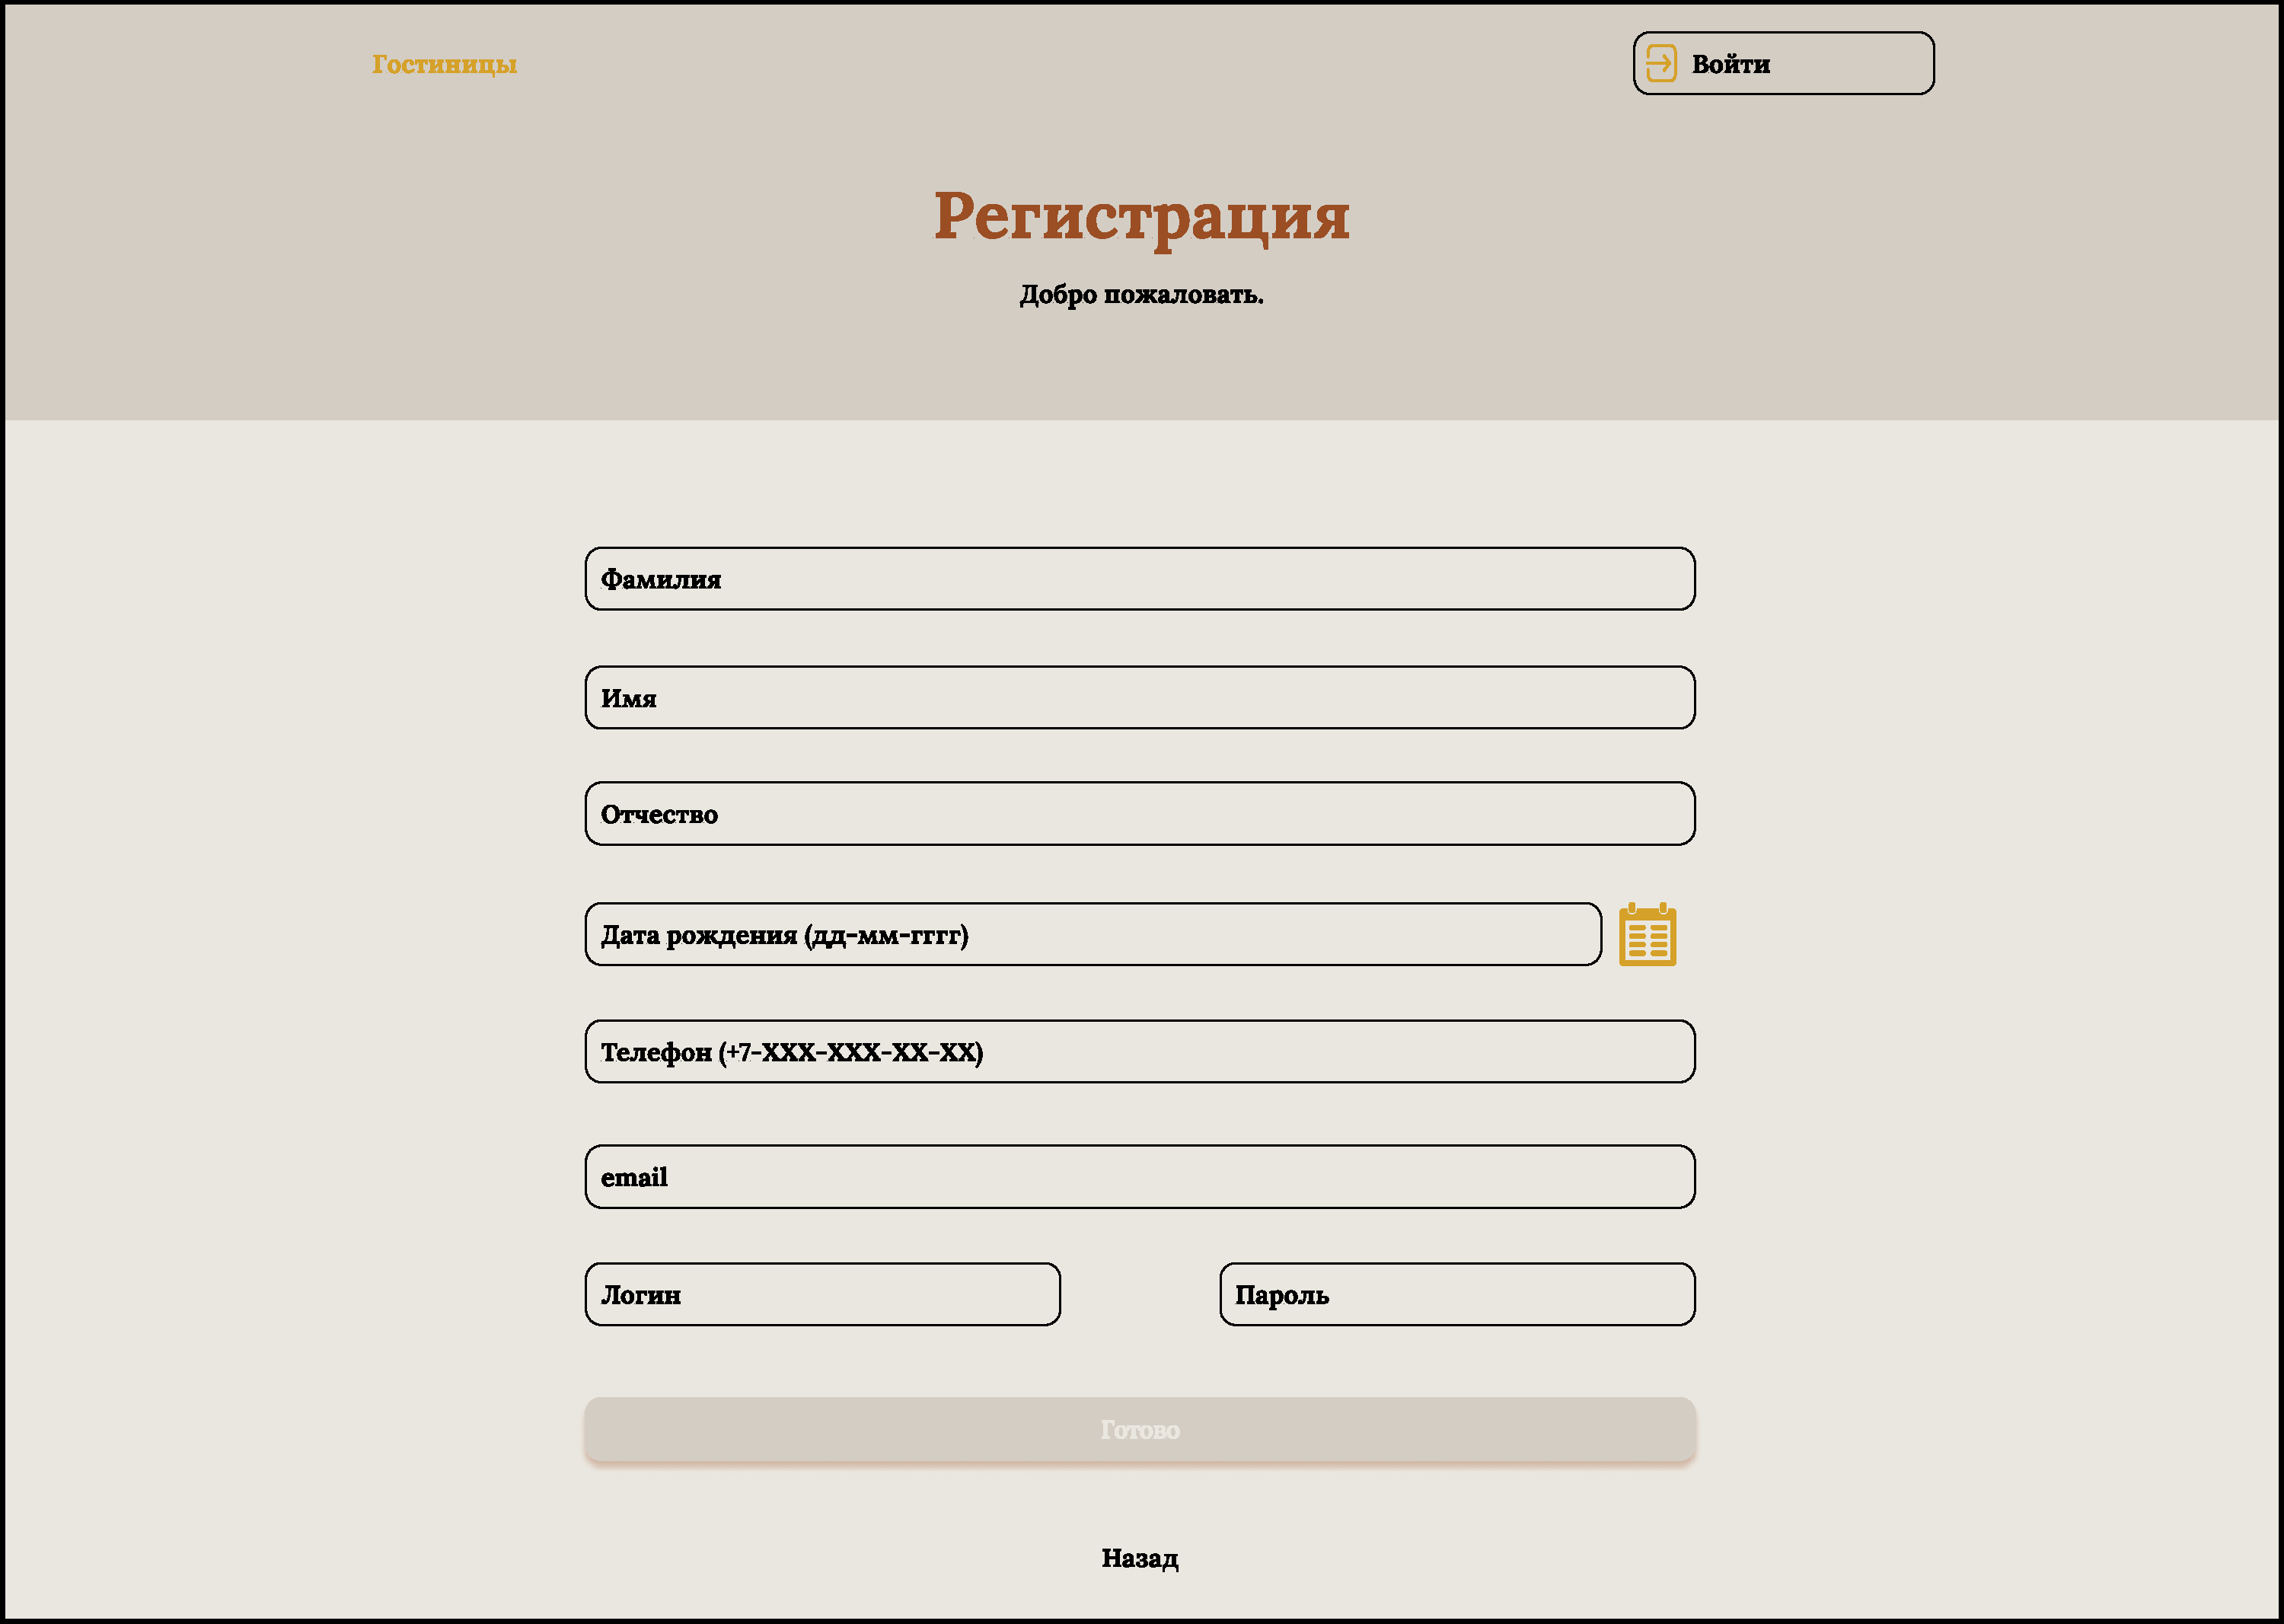
\includegraphics[scale = 0.3]{img/ui/registration.pdf}}
		\caption{Страница регистрации.}
		\label{fig:ui-reg}
	\end{center}
\end{figure} 

На рисунке \ref{fig:ui-hotels} изображена главная страница со списком гостиниц входящих в сеть. 

На сайте есть кнопка для входа в систему, поисковая строка, где пользователь может указать свои предпочтения, система будет производить поиск по ключевым словам из этого запроса и формировать подборку наиболее подходящих под описание гостиниц и номеров. Также есть уже готовые фильтры, достаточно нажать на интересующую характеристику.

\begin{figure}[h]
	\begin{center}
		{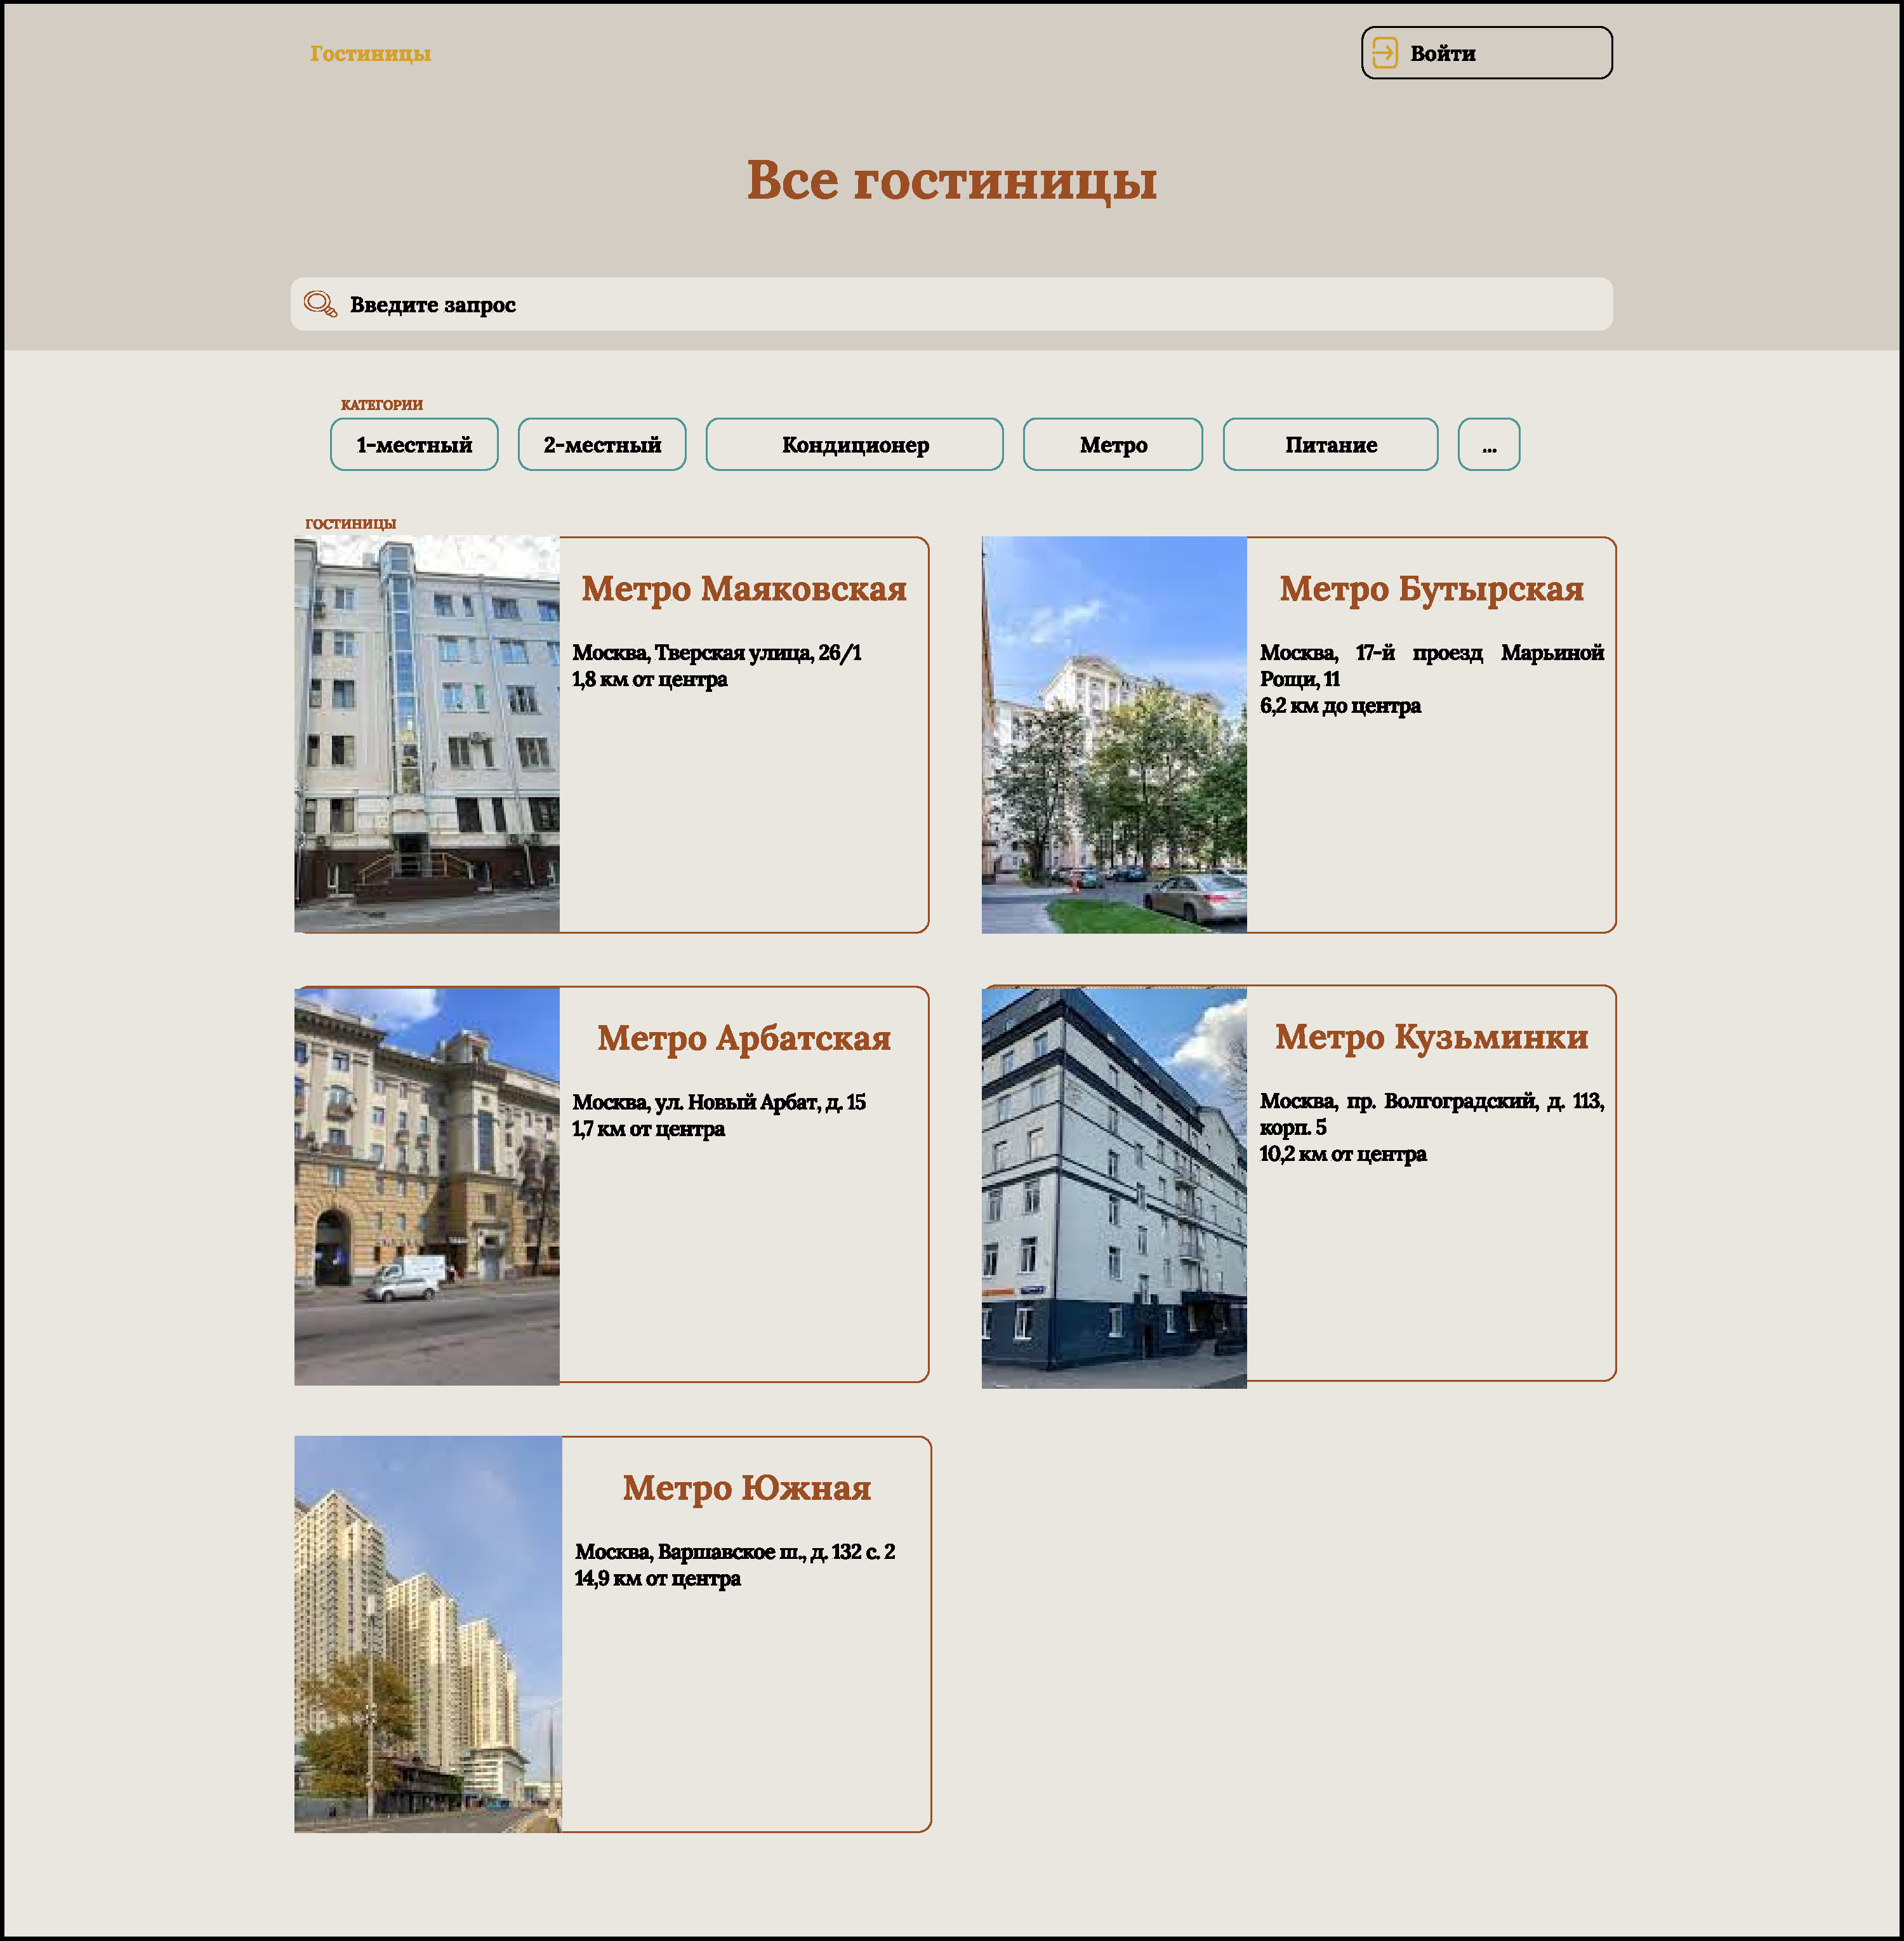
\includegraphics[scale = 0.3]{img/ui/hotels.pdf}}
		\caption{Диаграмма потоков данных при бронировании.}
		\label{fig:ui-hotels}
	\end{center}
\end{figure} 

\pagebreak

\section*{Физический дизайн}

\textbf{Выбор системы развертывания компонентов распределенной системы}


Требования для системы развёртывания компонентов.
\begin{itemize}
	\item \textbf{Изоляция}. Компоненты не  должны  иметь  доступа друг к другу, за исключением доступа, предусмотренного протоколом взаимодействия
	
	\item \textbf{Управление  ресурсами}. Компонент должен  потреблять  ограниченное  число  ресурсов  (процессорного  времени, оперативной памяти, места на жестком диске).
	
	\item \textbf{Отслеживание  зависимостей}.  Компонент  должен разворачиваться  монолитно  со  всеми  своими  библиотеками.  Это требование гарантирует, что компонент будет использоваться с теми же библиотеками, с которыми был протестирован.
	
	\item \textbf{Низкие накладные расходы}. Использование системы  развертывания не должно нести высокие накладные расходы для распределенной системы.
\end{itemize}

Полностью  удовлетворяет представленным требованиям такой инструмент  визуализации,  как  программа  \textit{Docker} \cite{bib:docker}.  Согласно определению,  Docker  —  программное  обеспечение  для  автоматизации развертывания и управления приложениями в среде виртуализации на уровне операционной системы Linux. Позволяет «упаковать» приложение со всем его окружением в контейнер, который может быть перенесен на любую Linux-систему, а также предоставляет  среду  по  управлению  контейнерами.  Разрабатывается  и  поддерживается одноименной компанией, распространяется как свободное программное обеспечение под лицензией Apache 2.0.

\textit{Контейнером}  называется  образ  изолируемой  части  Системы, содержащий приложение со всеми его зависимостями. В контейнере могут содержаться приложения и их среда выполнения: нужные библиотеки, конфигурационные файлы. Для облегчения работы используют единый репозиторий (хранилище) образов. Это позволяет применять уже готовые образы, которые необходимо только доработать для нужной задачи. Docker  эффективно используют для следующих задач:
\begin{itemize}
	\item тестирование распределённой системы;
	
	\item отслеживание зависимостей между компонентами разрабатываемой системы.
\end{itemize}

Преимуществами Docker по сравнению с виртуальными машинами (Oracle VM VirtualBox, Microsoft Hyper-V) являются:
\begin{itemize}
	\item низкие накладные расходы;
	
	\item наличие репозитория.
\end{itemize}

Использование программного обеспечения Docker позволит обеспечить высокую производительность при создании виртуальных вычислительных узлов и уменьшить потребление процессорных ресурсов. Недостатком Docker является то, что он работает только под ОС Linux. \\

\textbf{Выбор операционной системы}

Согласно требованиям технического задания, разрабатываемый портал должен обладать высокой доступностью, работать на типичных архитектурах ЭВМ (Intel x86, Intel x64), а так же быть экономически недорогим для сопровождения. Таким образом, требования к ОС следующие.
\begin{itemize}
	\item \textbf{Распространенность}. На рынке труда должно быть много специалистов, способных администрировать распределенную систему, работающую под управлением выбранной операционной системы.
	
	\item \textbf{Надежность}. Операционная система должна широко использоваться в стабильных проектах, таких как Mail.Ru, Vk.com, Google.com. Эти компании обеспечивают высокую работоспособность своих сервисов, и на их опыт можно положиться.
	
	\item \textbf{Наличие требуемого программного обеспечения}. Выбор операционной системы не должен ограничивать разработчиков в выборе программного обеспечения, библиотек.
	
	\item \textbf{Цена}.
\end{itemize}
 
Под данные требования лучше всего подходит ОС Ubuntu \cite{bib:ubuntu}. \textit{Ubuntu} — это дистрибутив, использующий ядро Linux. Как и все дистрибутивы Linux, Ubuntu является ОС с открытым исходным кодом, бесплатным для использования. Поставляется как в клиентской (с графическим интерфейсом), так и в серверной (без графического интерфейса) версиями. Ubuntu поставляется с современными версиями ПО. Преимуществом Ubuntu являются низкие требования к квалификации системных администраторов. Однако Ubuntu менее стабильна в работе. \\

\textbf{Выбор СУБД}

В  соответствии  с  техническим  заданием  разработка  бекенда предусматривает следующие требования.
\begin{itemize}
	\item \textbf{Безопасность  хранения  данных}.  Несанкционированный  доступ к данным клиентам должен быть невозможен.
	
	\item \textbf{Транзакционность}.  Должен  соблюдаться  принцип  «ACID» (Atomicity  —  Атомарность,  Consistency  —  Согласованность, Isolation — Изолированность, Durability — Надежность). Атомарность гарантирует, что транзакция не может быть зафиксирована частично.  Согласованность  —  что  успешное  завершение  транзакции оставит  систему  в  согласованном состоянии. Изолированность  —  что  параллельно  выполняемые  транзакции  не  будут влиять друг на друга. Надежность — что успешно завершенная транзакция  будет  зафиксирована,  а  в случае  сбоя, после восстановления системы, результаты транзакции не будут утеряны.
	
	\item \textbf{Масштабируемость}.  Выбранная  СУБД  должна  поддерживать репликацию, шардирование.
\end{itemize}

PostgreSQL \cite{bib:postgresql} -- реляционная  система  управления  базами данных. Она является  некоммерческим ПО с открытым исходным кодом. Для работы с этой СУБД существуют библиотеки для таких распространенных  языков  программирования,  как  Python,  Ruby, Perl, PHP, C, C++, Java, C\#, Go. Она работает под управлением многих операционных систем: Linux, MacOS, Windows, FreeBSD, Solaris и  др. По сравнению с MySQL система PostgreSQL лучше работает с репликацией, так как в ней существует журнал (средство восстановления системы  в случае  сбоя) физической модификации страниц. PostgreSQL осуществляет асинхронную репликацию типа «ведущий — ведомый».

Выбор  СУБД  PostgreSQL  для  хранения  данных разрабатываемой системы обеспечит надежность, безопасность и масштабируемость. \\

\textbf{Выбор языка разработки компонент портала}

Исходя из приведенных требований к системе, можно выявить следующие требования к языку программирования.

\begin{itemize}
	\item \textbf{Наличие  разнообразных  библиотек}.  Использование  готовых библиотек ускоряет разработку программного обеспечения. Также важно, что благодаря использованию распространенных оттестированных библиотек снижается  вероятность  ошибки.  Это повышает надежность  программного  обеспечения.
	
	\item \textbf{Совместимость с выбранными ранее технологиями}. Выбранный  язык  должен  уметь  взаимодействовать  с  ОС  Linux,  СУБД PostgreSQL.
	
	\item \textbf{Высокая скорость разработки}. На  ранних  этапах разработки портала технические требования часто меняются. Язык программирования должен позволять как можно быстрее  вносить изменения в коды программ.
\end{itemize}

Под данные требования хорошо подходит язык Java \cite{bib:java}. Это универсальный объектно-ориентированный язык со строгой типизацией. В нём реализован принцип WORA (от английского: write once, run anywhere). Это позволяет запускать приложения везде, где есть среда исполнения JRE (от английского: Java Runtime Environment). При этом не имеет значения, какая операционная система установлена на устройстве.

У Java есть ряд преимуществ.
\begin{itemize}
	\item \textbf{Простота} -- чёткие синтаксические правила и понятная семантика.
	
	\item \textbf{Объектно-ориентированный подход}.
	
	\item \textbf{Безопасность}. Обойти или взломать механизмы защиты крайне сложно.
	
	\item \textbf{Производительность}. Новые версии динамических компиляторов Java не уступают традиционным из других платформ. При необходимости \, те или иные \, приёмы оптимизации \, включаются или отменяются \, JIT-компилятором.
	
	\item \textbf{Надёжность}. Компилятор способен выявить ошибки ещё до выполнения кода, то есть на ранних стадиях.
	
	\item \textbf{Независимость от аппаратной части и ОС}. Важно лишь наличие исполняющей среды и JVM. Байт-код легко интерпретируется на любой машине. Кроссплатформенностью отличается также интерфейс, реализованный в системных библиотеках.
	
	\item \textbf{Динамичность и адаптируемость}. При необходимости можно добавить в библиотеки новые объекты, методы.
	
	\item \textbf{Удобные и эффективные сетевые возможности}. Приложения умеют находить объекты в сети и открывать к ним доступ. Предоставляется обширная программная библиотека для передачи данных по самым распространённым протоколам: FTP, HTTP, TCP/IP. Работает механизм вызова удалённых методов. \\
\end{itemize}

\textbf{Выбор фреймворка для разработки портала}

К выбору фреймворка предъявляют те же требования, что и к выбору языка программирования:
\begin{itemize}
	\item большое число стандартных возможностей;
	
	\item совместимость с выбранными ранее технологиями;
	
	\item высокая скорость разрабатываемого портала.
\end{itemize}

Для  разработки  <<Распределённой системы бронирования номеров гостиниц сети Apartlux>> должны быть использованы  фреймворки,  основанные  на парадигме MVC:
\begin{itemize}
	\item модель представляет объекты, хранимые в системе: информацию об аккаунтах, гостиницах, номерах, бронированиях;
	
	\item вид  отвечает  за  визуализацию  моделей;
	
	\item элемент управления отвечает за взаимодействие пользователя и программного обеспечения.
\end{itemize}

\textit{Spring Boot} \cite{bib:spring} — это фреймворк на основе Java с открытым исходным кодом. Благодаря быстродействию и простоте работы он стал популярным решением для создания развертываний в виде архива веб-приложений (WAR) и автономных Java-приложений.

Он позволяет избавиться от трудоемкой первоначальной установки и настройки среды развертывания. Основные преимущества:
\begin{itemize}
	\item быстрая и легкая разработка приложений;
	
	\item автоконфигурация всех компонентов;
	
	\item готовые встроенные серверы, обеспечивающие ускоренное и более продуктивное развертывание приложений;
	
	\item отсутствие конфигурации XML;
	
	\item большой выбор плагинов, облегчающих работу со встроенными базами данных, легкий доступ к ним и службам очередей.
	
	\item подробная документация.
\end{itemize}

К недостаткам этого фреймворка относятся:
\begin{itemize}
	\item создает множество неиспользуемых зависимостей, что приводит к большому размеру файла развертывания;
	
	\item не подходит для создания монолитных приложений.
\end{itemize}

Таким образом, в результате проведённого анализа в качестве системы развёртывания компонентов был выбран Docker, ОС -- Ubuntu, СУБД -- PostgreSQL, язык программирования -- Java, фреймворк -- Spring Boot. \\

\textbf{Обеспечение надежности портала}

В рассматриваемой <<Распределённой системе бронирования номеров гостиниц сети Apartlux>> для  обеспечения надежности функционирования СУБД  будет применяться  репликация типа «ведущий – ведомый» и шардинг. Для обеспечения надежности данных СУБД необходимо разработать скрипт для автоматического создания резервной копий базы данных по расписанию.

Для фронтенда и бекендов целесообразно применить зеркалирование. Это обеспечит отказоустойчивость системы: в случае сбоя любого из ее узлов запросы на чтение данных будут выполняться. 

Отказоустойчивость фронтенда возможно за счет его зеркалирования на несколько серверов. Выбор одного из зеркалируемых серверов осуществля-ется с помощью прописывания в DNS (система доменных имен) записях адресов всех серверов, на которых располагаются фронтенды. 

Также должна быть настроена система мониторинга на предмет возникновения ошибок в системе, в случае их появления оповещение должно придти в Telegram-канал для наиболее оперативного реагирования.\\

